\chapter{Methods}
\label{chap:phage_methods}

This chapter introduces the reaction-diffusion model used in this project, explaining the necessary coupling terms to describe bacteria-phage interactions and the non-dimensional version of it. Then we will introduce the chemostat version of it, used to model an analogous system in a well-mixed environment. Furthermore, we will introduce the respective observables which were defined to quantify results obtained from the ensuing dynamics.
\section{Model}
\begin{figure}
\centering
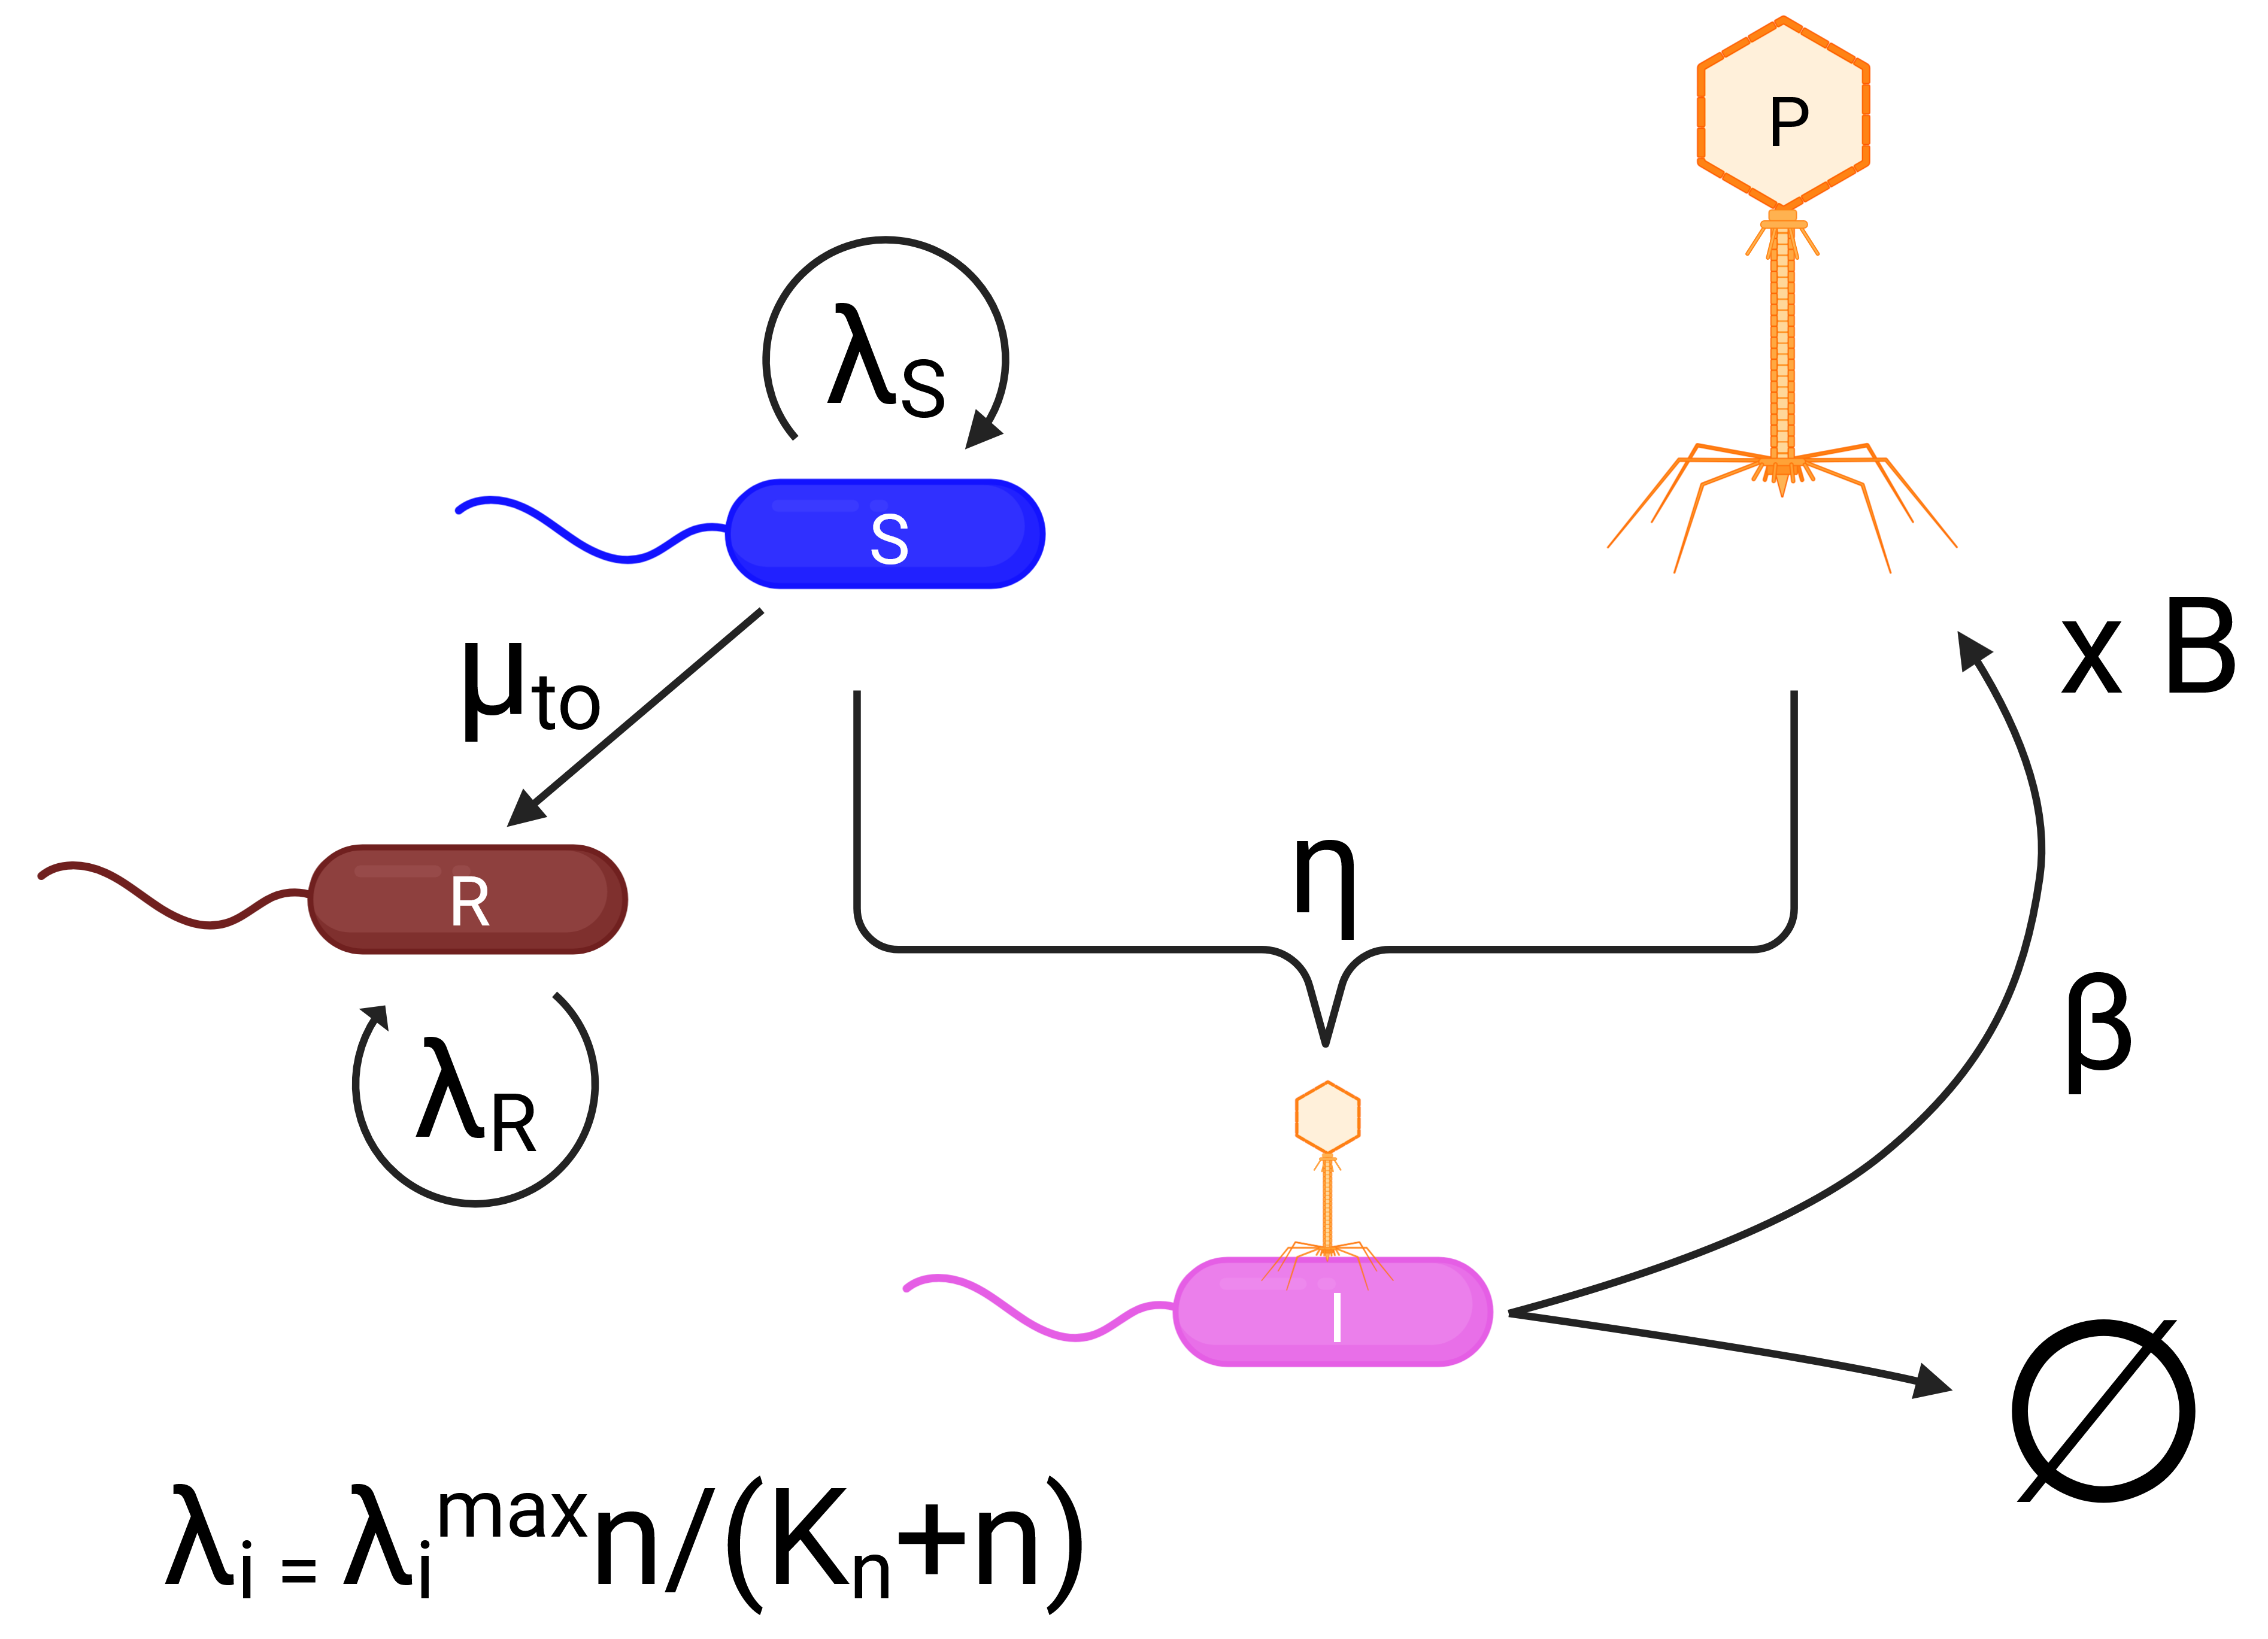
\includegraphics[width=\linewidth]{graphics/2025_09_30_phages_fig1.png}
\caption{\textbf{Interactions within the reaction-diffusion model describing bacteria-phage interactions} Sensitive bacteria, depicted in blue, grow with a growth rate $\lambda_s$ and are infected by phages, depicted in orange, with an infection rate $\eta$. This infection process forms infected bacteria, depicted in pink, which burst with a burst rate $\beta$ and upon lysis release $B$ new phages. In addition, resistant bacteria, depicted in brown, are present in the system, grow with a growth rate $\lambda_r$ and sensitive bacteria can mutate to become resistant with mutation rate $\mu_{to}$. Both growth rates are changing depending on nutrient availability.}
\label{fig:model_sketch}
\end{figure}
Inspired by models from previous works~\cite{Ping2020-vd, Claydon2021-cu}, we build a model to simulate bacteria-phage interactions for a lytic phage taking resistant bacteria and nutrient competition into account. The interactions between components in our model are graphically depicted in Figure \ref{fig:model_sketch} while excluding diffusion and nutrients in the sketch for simplicity. Components in our model are the densities of sensitive bacteria, $S(x,t)$, infected bacteria, $I(x,t)$, resistant bacteria, $R(x,t)$, phages, $P(x,t)$ and of nutrients, $n(x,t)$. The following set of~\gls{pde}s in one space dimension $x$ and time $t$ defines our model:
\begin{align}
    \frac{\text{d}S}{\text{d}t} = D_b &\frac{\partial^2S}{\partial x^2} + \left( 1 - \mu_{to} \right) \lambda_s S \frac{n}{K_n+n}  - \eta SP \\
    \frac{\text{d}I}{\text{d}t} = D_b &\frac{\partial^2I}{\partial x^2} + \eta SP - \beta I\\
    \frac{\text{d}R}{\text{d}t} = D_r &\frac{\partial^2R}{\partial x^2} + \left[\lambda_r R + \mu_{to} \lambda_s S \right] \frac{n}{K_n+n}\\
    \frac{\text{d}P}{\text{d}t} = D_p &\frac{\partial^2P}{\partial x^2} + \beta BI - \eta P(S+I) \\
    \frac{\text{d}n}{\text{d}t} = D_n &\frac{\partial^2n}{\partial x^2} - \frac{1}{Y} \left( \lambda_s S + \lambda_r R \right) \frac{n}{K_n+n}
\end{align}
where $D_b$, $D_p$, $D_r$ and $D_n$ are the respective diffusion rates, $\mu_{to}$ is the mutation rate, $\lambda_s$ and $\lambda_r$ are the respective growth rates, $K_n$ is the half-velocity constant, $\eta$ is the infection rate, $\beta$ is the lysis rate, $B$ is the burst size and $Y$ is the nutrient yield. To improve readability, we omit dependencies on space and time for all components. It is possible to generalize this model to multiple dimensions, but we focus on a one-dimensional scenario.

We non-dimensionalize the model using the following transformations for space, time and component densities:\\
% \begin{align*}
%     x &\rightarrow \tilde{x} = \sqrt{\frac{D_b}{\lambda_s}} x \\
%     t &\rightarrow \tilde{t} = \frac{1}{\lambda_s} \\
%     S &\rightarrow \tilde{S} = K_n Y S \\
%     I &\rightarrow \tilde{I} = K_n Y I \\ 
%     R &\rightarrow \tilde{R} = K_n Y R \\
%     P &\rightarrow \tilde{P} = \frac{\lambda_s}{\eta} P \\
%     n &\rightarrow \tilde{n} = K_n n
% \end{align*}
$x \rightarrow \tilde{x} = \sqrt{\frac{D_b}{\lambda_s}} x$; $t \rightarrow \tilde{t} = \frac{1}{\lambda_s}$; \\
$S \rightarrow \tilde{S} = K_n Y S$; $I \rightarrow \tilde{I} = K_n Y I$; $R \rightarrow \tilde{R} = K_n Y R$; $P \rightarrow \tilde{P} = \frac{\lambda_s}{\eta} P$; $n \rightarrow \tilde{n} = K_n n$\\
When redefining the parameters as:\\
% \begin{align*}
%     \tilde{D_p} &= \frac{D_p}{D_b} \\
%     \tilde{D_r} &= \frac{D_r}{D_b} \\
%     \tilde{D_n} &= \frac{D_n}{D_b} \\
%     \tilde{\beta} &= \frac{\beta}{\lambda_s} \\
%     \tilde{\eta} &= \frac{\eta K_n Y}{\lambda_s} \\
%     \tilde{\lambda_r} &= \frac{\lambda_r}{\lambda_s} \\
%     \tilde{B} &= B
% \end{align*}
$\tilde{D_p} = \frac{D_p}{D_b}$; $\tilde{D_r} = \frac{D_r}{D_b}$; $\tilde{D_n} = \frac{D_n}{D_b}$; $\tilde{\beta} = \frac{\beta}{\lambda_s}$; $\tilde{\eta} = \frac{\eta K_n Y}{\lambda_s}$; $\tilde{\lambda_r} = \frac{\lambda_r}{\lambda_s}$; $\tilde{B} = B$;\\
we can write the non-dimensionalized set of coupled~\gls{pde}s, dropping the tildes, as:
\begin{align}
    \frac{\text{d}S}{\text{d}t} &= \frac{\partial^2S}{\partial x^2} + \left( 1 - \mu_{to} \right) S \frac{n}{1+n}  - SP \\
    \frac{\text{d}I}{\text{d}t} &= \frac{\partial^2I}{\partial x^2} + SP - \beta I\\
    \frac{\text{d}R}{\text{d}t} &= D_r \frac{\partial^2R}{\partial x^2} + \left[\lambda_r R + \mu_{to} S \right] \frac{n}{1+n}\\
    \frac{\text{d}P}{\text{d}t} &= D_p \frac{\partial^2P}{\partial x^2} + \beta \eta BI - \eta P(S+I) \\
    \frac{\text{d}n}{\text{d}t} &= D_n \frac{\partial^2n}{\partial x^2} - \left( S + \lambda_r R \right) \frac{n}{1+n}
\end{align}
For the well-mixed, liquid, scenario, we drop the diffusion terms, add chemostat balancing terms and after analogous non-dimensionalization, we obtain the following set of~\gls{ode}:
\begin{align}
    \frac{\text{d}S}{\text{d}t} &= \left( 1 - \mu_{to} \right) S \frac{n}{1+n}  - SP - d S\\
    \frac{\text{d}I}{\text{d}t} &= SP - \beta I - d I\\
    \frac{\text{d}R}{\text{d}t} &= \left[\lambda_r R + \mu_{to} S \right] \frac{n}{1+n} - d R\\
    \frac{\text{d}P}{\text{d}t} &= \beta \eta BI - \eta P(S+I) -d P\\
    \frac{\text{d}n}{\text{d}t} &= - \left( S + \lambda_r R \right) \frac{n}{1+n} - d n
\end{align}
Inspired by experimental values, used also by other models~\cite{Marchi2025-yu, Claydon2021-cu}, we use for our parameters in the non-dimensionalized system, the parameter set given in table~\ref{tab:model_parameters}, unless specified otherwise.
\begin{table}
    \centering
    \begin{tabular}{c|c|c}
         parameter & chemostat & one-dimensional \\ \hline
         $D_p$& 0.0 & 1/18\\ 
         $D_r$& 0.0 & 1.0\\ 
         $D_n$& 0.0 & 50/3\\ 
         $\beta$& 50/13 & 50/13\\ 
         $\lambda_r$& 1.0 & 1.0\\ 
         $B$& 70 & 70\\ 
         $\eta$& 2/65 & 2/65\\ 
         $\mu_{to}$& 0.01 & 0.01
    \end{tabular}
    \caption{Standard parameter values used in the model}
    \label{tab:model_parameters}
\end{table}

Numerical simulations of the equations were performed in python, using \text{scipy.solve\_ivp()} with a flexible time step up to a time $t_{max}$, using a discretization of space with $N$ discretization points and stepping size $dx$. For the non-dimensionalized simulation space, we use the parameters given in table~\ref{tab:spacetime_parameters}, unless specified otherwise.

\begin{table}
    \centering
    \begin{tabular}{c|c|c}
         parameter & chemostat & one-dimensional \\ \hline
         $t_{max}$& 20000.0 & 910.0\\ 
         $N$& 1 & 600\\ 
         $dx$& 0.0 & $\sqrt{65}$/6
    \end{tabular}
    \caption{Simulation parameters used to solve the model}
    \label{tab:spacetime_parameters}
\end{table}

\section{Observables}
\begin{figure}
\centering
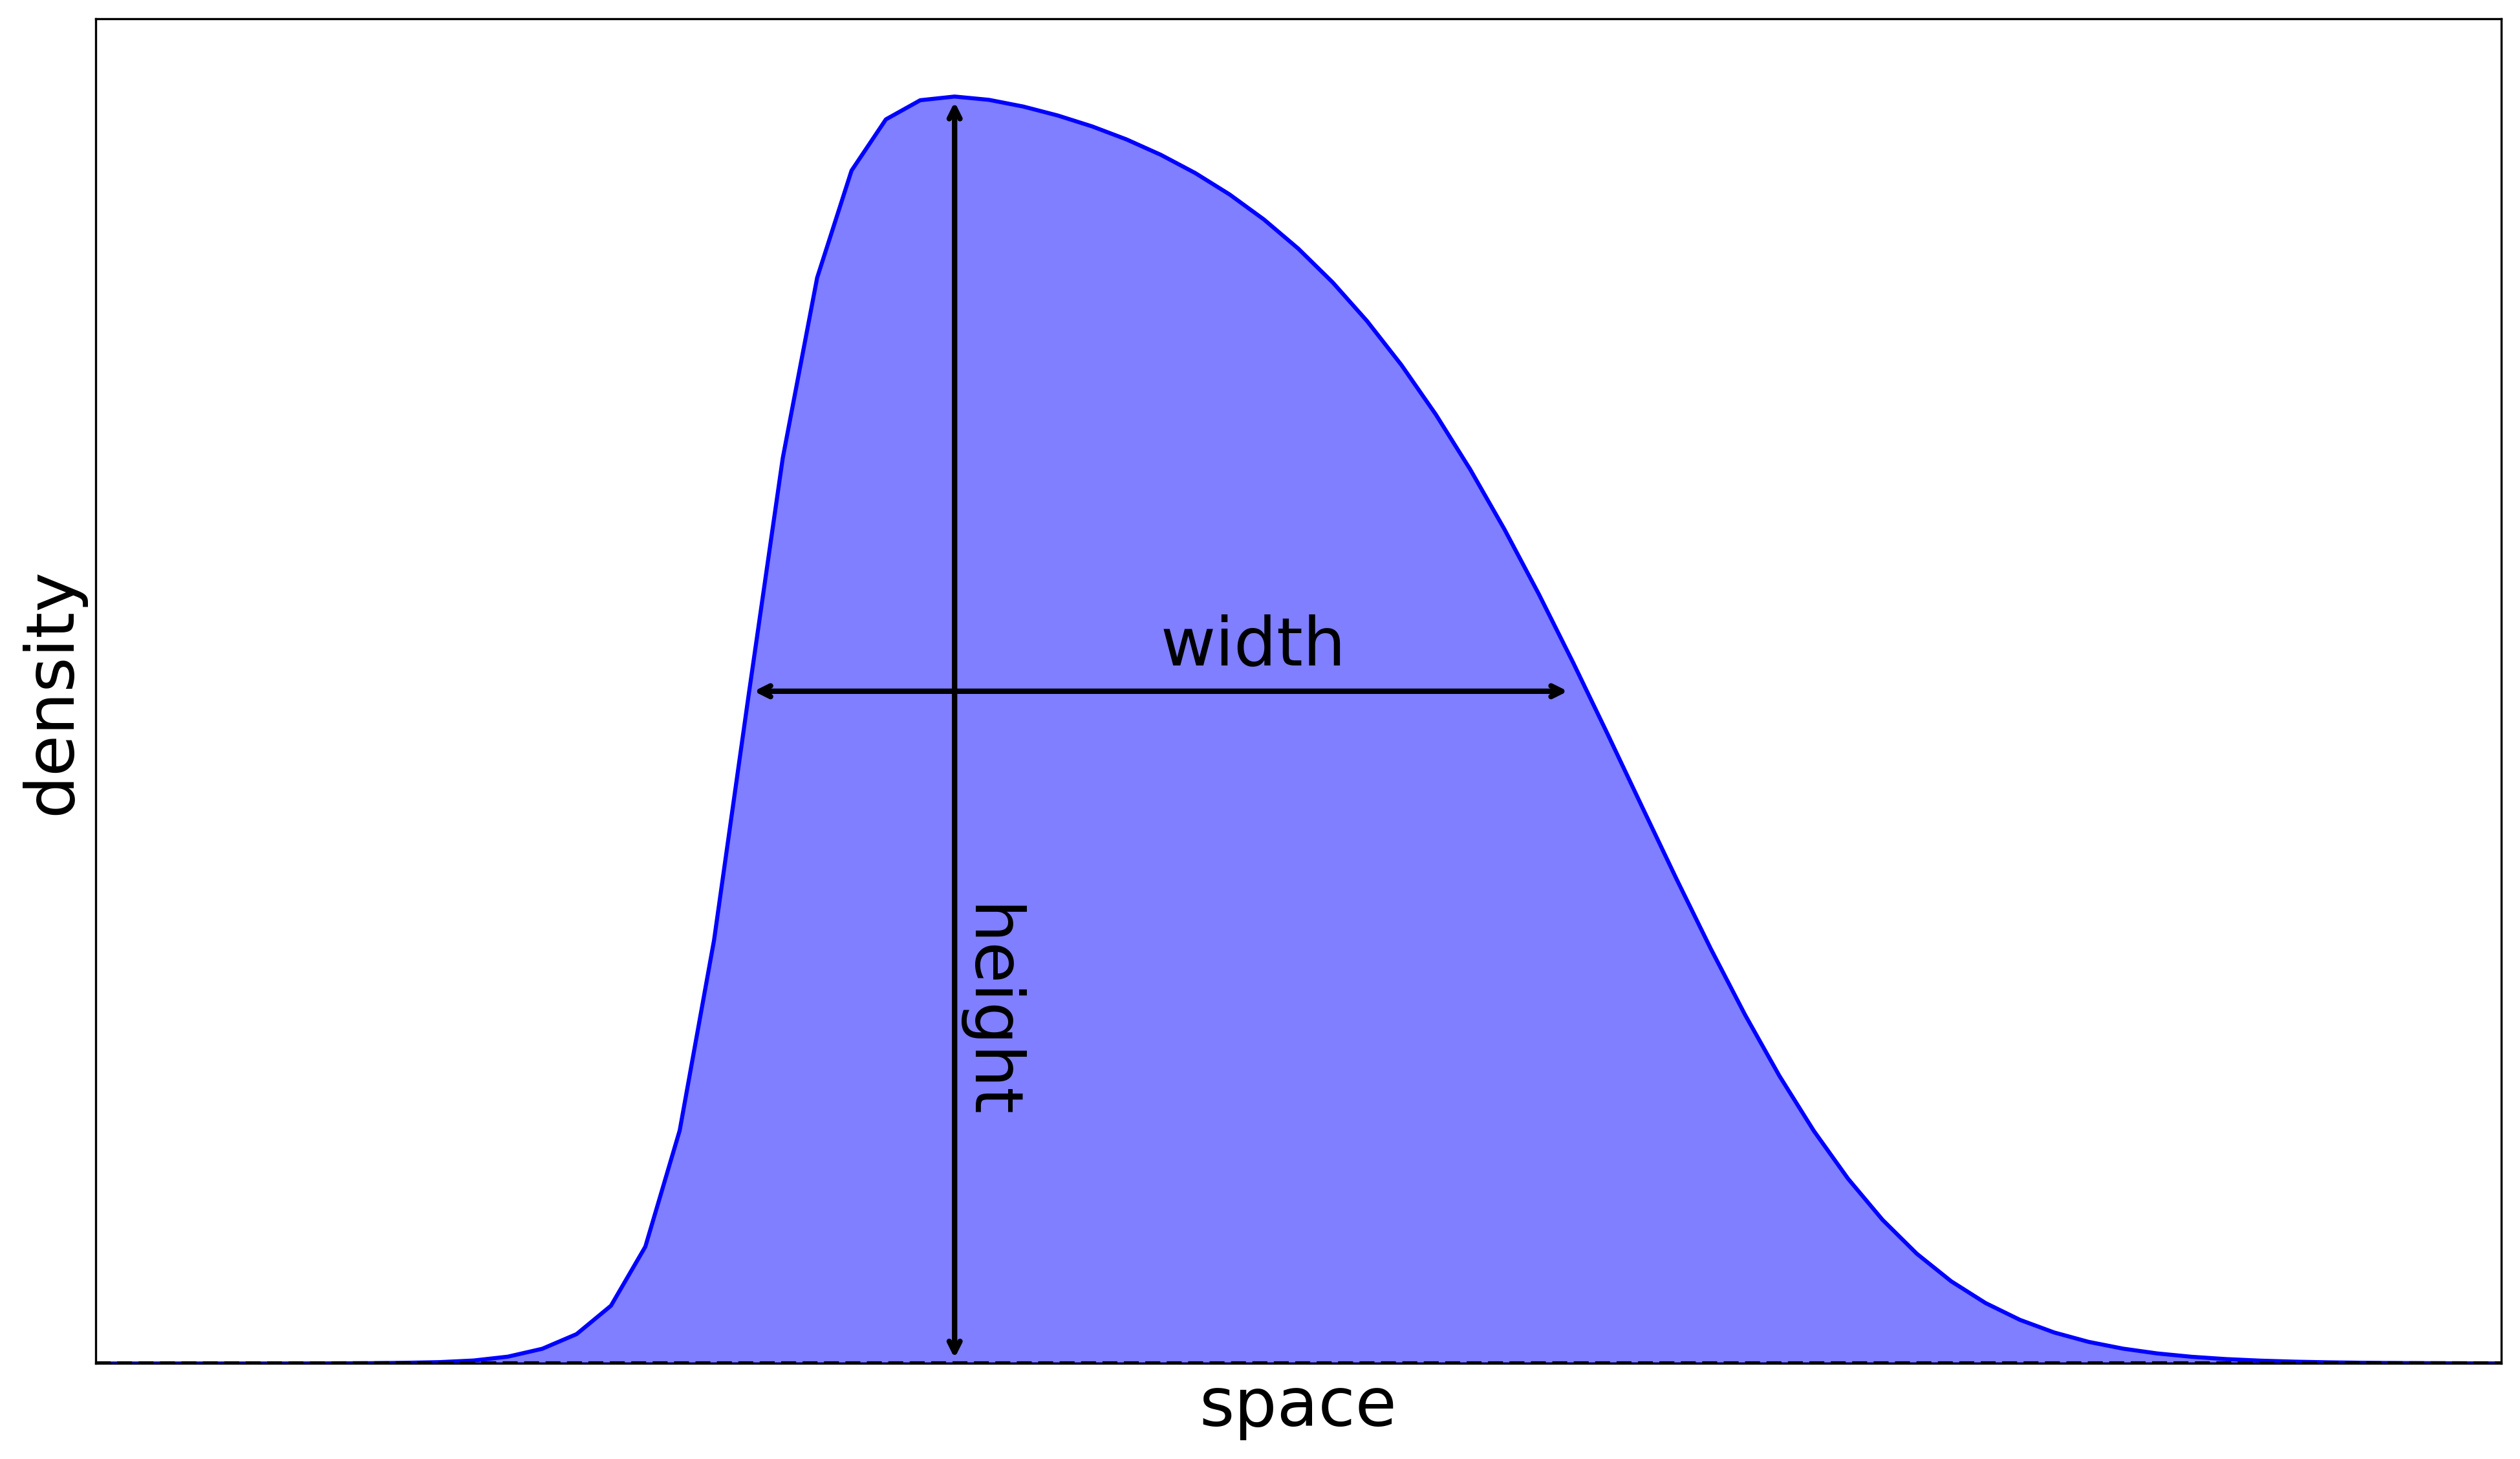
\includegraphics[width=\linewidth]{graphics/2025_09_30_phages_fig2.png}
\caption{\textbf{Explanation of observables to quantify dynamics of the reaction-diffusion model} The shaded area is the amount of bacteria or phages we measure and in addition the maximum of the wave is measured as the height and the width is measured at $10^{-6}$ of the maximum. Here the width is shown at $0.5$ of the maximum to improve visibility.}
\label{fig:observable_sketch}
\end{figure}
The model forms traveling waves as a steady state solution and we describe and quantify those waves using three observables. We measure the amount of bacteria which is represented as the area under the curve and additionally we measure the height at the maximum and the width at $10^{-6}$ of the maximum of the curve as shown in Figure~\ref{fig:observable_sketch}.
